\documentclass[french,twoside,openany,showtrims]{root/support/latex/sbabook/sbabook}

\usepackage{url} % define and apply style to URLs
\def\url@sfstyle{\def\UrlFont{\sf}}
\urlstyle{sf}
\usepackage[unicode,breaklinks,hidelinks]{hyperref} % undecorated hyperlinks
\usepackage{wrapfig}
\usepackage{graphicx}

\title{Rapport hebdomadaire de stage - Semaine 1}
\author{Yann Dubois}
\date{\today}

\hypersetup{pdfinfo = {
    Title = {\thetitle},
    Author = {\theauthor},
    Keywords = {LaTeX, document class, book, typography}}}

\newcommand\hrefnote[3][]{% inline linked text, plus URL in footnote
  % \hrefnote[]{URL}{link text}
  \href{#2}{#3}\footnote{\url{#2} #1}}

\begin{document}
  \maketitle
  \pagestyle{titlingpage}
  \thispagestyle{titlingpage}

  \vskip10em
  
\includegraphics{root/figures/logo_INRIA.png}
  \hskip10em
  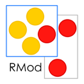
\includegraphics[scale=2.0]{root/figures/rmod.png}
  \vskip0em
  \hskip0em

  \chapter{Le stage}
    \section{L'entreprise}
      Le stage se déroule à l'\hrefnote{http://www.inria.fr/}{INRIA} avec une équipe
      de recherche du nom de \hrefnote{http://rmod.inria.fr/web/}{RMod}. Son but est de
      soutenir la remodularisation et le développement d'applications modulaires
      orientées objet. L'équipe est constituée d'une vingtaine de personnes et est menée
      par \hrefnote[ --- Page de Stéphane DUCASSE]{http://rmod.inria.fr/web/team/ducasse}{Stéphane Ducasse}.
      L'équipe étant experte en programmation de langage dynamique, ils développent
      l'environnement de développement \hrefnote{http://pharo.org/}{Pharo} et
      l'utilise dans des cas réel lors de la création de logiciels et d'outils
      pour Pharo. L'une des personne contribuant à se projet est Damien CASSOU,
      mon tuteur de stage.

    \section{Le tuteur de stage}
      \begin{wrapfigure}[4]{r}{2cm}
        
\includegraphics[width=2cm]{root/figures/week1/damien_cassou.jpg}
      \end{wrapfigure}
      Damien CASSOU\\
      Poste : Enseignant Chercheur\\
      Téléphone : 03 59 35 87 49\\
      email: damien.cassou@inria.fr\\

      \newpage
      Damien est maître de conférence à l'université de Lille 1 et chercheur en informatique, ses recherches
      portent sur les langages de programmation dynamique (entre autre les traits
      et les modules). Avec l'aide de Pharo, il a créé un transformateur open-source
      de texte. Ce transformateur se nomme \hrefnote{https://github.com/pillar-markup}{Pillar},
      il prend des fichier *.pillar en entrée et en sort des fichiers dans d'autres
      langages comme le HTML ou le \LaTeX{}.

    \section{La mission}
      \paragraph{Thème: Restructuration et développement}

      \paragraph{Nature(étude, audit,analyse,développement, maintenance ...) : analyse, développement et maintenance}

      ~~\\
      ~~\\

      Pillar est un format textuel simple et concis. Pillar est aussi un logiciel
      libre (licence MIT), écrit en Pharo, permettant de convertir un texte Pillar
      en un fichier PDF, HTML ou Markdown (d'autres formats de sorties sont prévus
      comme DocBook et AsciiDoc).\\

      ~~\\

      Pillar est notamment utilisé pour écrire des livres (Dynamic Web Development,
      Enterprise Pharo et Updated Pharo by Example). Pillar a récemment été utilisé
      comme langage source pour la réalisation du \hrefnote{https://www.fun-mooc.fr/courses/inria/41010/session01/about}{MOOC Pharo} :
      description de la structure du MOOC, slides et feuilles d'exercices ont tous été écrit avec Pillar.\\

      ~~\\

      La création d'un nouveau projet de documentation en Pillar est une activité
      complexe, non documentée et qui nécessite beaucoup de copier/coller de projets
      existants. Le projet \hrefnote{https://github.com/pillar-markup/book-skeleton/}{book-skeleton}
      a été crée pour résoudre le problème mais cette solution souffre d'autres problèmes
      (\url{https://github.com/pillar-markup/pillar/issues/68}). La mission principale de ce
      stage sera de faciliter ce processus en proposant la création automatique de nouveaux
      projets en fonction de quelques templates de projets fournis (livre, slides de cours,
      documentation courte, ...) dans le même style que maven archetypes. Ce travail
      se fera en collaboration avec Thibault, un autre stagiaire, dont le rôle sera
      de simplifier Pillar pour se rappocher du style pipe\&filter d'unix.\\

      ~~\\

      Au delà de ça, l'étudiant travaillera à la restructuration des paquetages Pillar
      pour supprimer les dépendances cycliques. Il veillera aussi à empêcher l'introduction
      de nouvelles dépendances cycliques grâce à une configuration du serveur d'intégration
      continue et de l'outil de chargement de code Pharo.\\

      ~~\\

      Les tâches ci-dessus se feront dans un environnement où Pillar est déjà utilisé
      par une communauté qui ne manquera pas de soulever des problèmes et remonter
      des besoins. L'étudiant devra prendre en compte ces retours pendant toute
      la durée de son stage.\\

      ~~\\

      Bénéfices de ce stage pour l'étudiant :\\

      \begin{itemize}
        \item Découverte d'un nouveau langage de programmation et de son environnement de développement innovant
        \item Mise en pratique des principes de conception objets et de l'écriture de tests
        \item Développement d'un outil utilisé par une communauté qui soulève régulièrement
        des problèmes ou remonte des besoins (75 tickets ouverts actuellement)
        \item Intégration dans un groupe de recherche anglophone passionné de programmation
      \end{itemize}

      Durée prévisionnelle: 5 mois\\
      Taille du projet: 299 classes, 2846 méthodes, 14088 lignes de code\\
      Technologie: Pharo, Jenkins, Git, Bash\\
      Langages, support de développement: Pharo, Smalltalk

      \section{Pour résumé}
      \begin{itemize}
        \item Correction des bugs, amélioration de Pillar
        \item Ajout d'un exporter vers Scenarii (un langage resemblant à XML)
        \item Proposition de nouvelle fonctionnalité
        \item Communication avec la communauté pour comprendre les problèmes
      \end{itemize}

\clearpage

\end{document}
